% !TeX spellcheck = en_GB
% !TeX program = pdflatex
%
% LetzCV-sleek 1.0 LaTeX template
% Author: Andreï V. Kostyrka, University of Luxembourg
%
% This template fills the gap in the available variety of templates
% by proposing something that is not a custom class, not using any
% hard-coded settings deeply hidden in style files, and provides
% a handful of custom command definitions that are as transparent as it gets.
% Developed at the University of Luxembourg.
%
% *NOTHING IS HARCODED, and never should be.*
%
% Target audience: applicants in the IT industry, or business in general
%
% The main strength of this template is, it explicitly showcases how
% to break the flow of text to achieve the most flexible right alignment
% of dates for multiple configurations.

\documentclass[12pt, a4paper]{article} 

\usepackage[T1]{fontenc}     % We are using pdfLaTeX,
\usepackage[utf8]{inputenc}  % hence this preparation
\usepackage[british]{babel}  
\usepackage[left = 0mm, right = 0mm, top = 0mm, bottom = 0mm]{geometry}
\usepackage[stretch = 25, shrink = 25]{microtype}  
\usepackage{graphicx}        % To insert pictures
\usepackage{xcolor}          % To add colour to the document
\usepackage{marvosym}        % Provides icons for the contact details

\usepackage{enumitem}        % To redefine spacing in lists
\setlist{parsep = 0pt, topsep = 0pt, partopsep = 1pt, itemsep = 1pt, leftmargin = 6mm}

\usepackage{FiraSans}        % Change this to use any font, but keep it simple
\renewcommand{\familydefault}{\sfdefault}

\definecolor{cvblue}{HTML}{304263}

%%%%%%% USER COMMAND DEFINITIONS %%%%%%%%%%%%%%%%%%%%%%%%%%%
% These are the real workhorses of this template
\newcommand{\dates}[1]{\hfill\mbox{\textbf{#1}}} % Bold stuff that doesn’t got broken into lines
\newcommand{\is}{\par\vskip.5ex plus .4ex} % Item spacing
\newcommand{\smaller}[1]{{\small$\diamond$\ #1}}
\newcommand{\headleft}[1]{\vspace*{3ex}\textsc{\textbf{#1}}\par%
    \vspace*{-1.5ex}\hrulefill\par\vspace*{0.7ex}}
\newcommand{\headright}[1]{\vspace*{2.5ex}\textsc{\Large\color{cvblue}#1}\par%
     \vspace*{-2ex}{\color{cvblue}\hrulefill}\par}
%%%%%%%%%%%%%%%%%%%%%%%%%%%%%%%%%%%%%%%%%%%%%%%%%%%%%%%%%%%%

\usepackage[colorlinks = true, urlcolor = red, linkcolor = white]{hyperref}

\begin{document}

% Style definitions -- killing the unnecessary space and adding the skips explicitly
\setlength{\topskip}{0pt}
\setlength{\parindent}{0pt}
\setlength{\parskip}{0pt}
\setlength{\fboxsep}{0pt}
\pagestyle{empty}
\raggedbottom

\begin{minipage}[t]{0.36\textwidth} %% Left column -- outer definition
%  Left column -- top dark rectangle
\colorbox{cvblue}{\begin{minipage}[t][5mm][t]{\textwidth}\null\hfill\null\end{minipage}}

\vspace{-.2ex} % Eliminates the small gap
\colorbox{cvblue!90}{\color{white}  %% LEFT BOX
\kern0.09\textwidth\relax% Left margin provided explicitly
\begin{minipage}[t][293mm][t]{0.82\textwidth}
\raggedright
\vspace*{2.5ex}

\Large Quentin \textbf{\textsc{Moreno-Gelos}} \normalsize 

% Centering without extra vertical spacing
% \null\hfill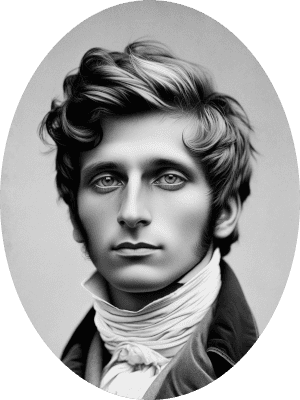
\includegraphics[width=0.65\textwidth]{oval-transparent.png}\hfill\null

% \null\hfill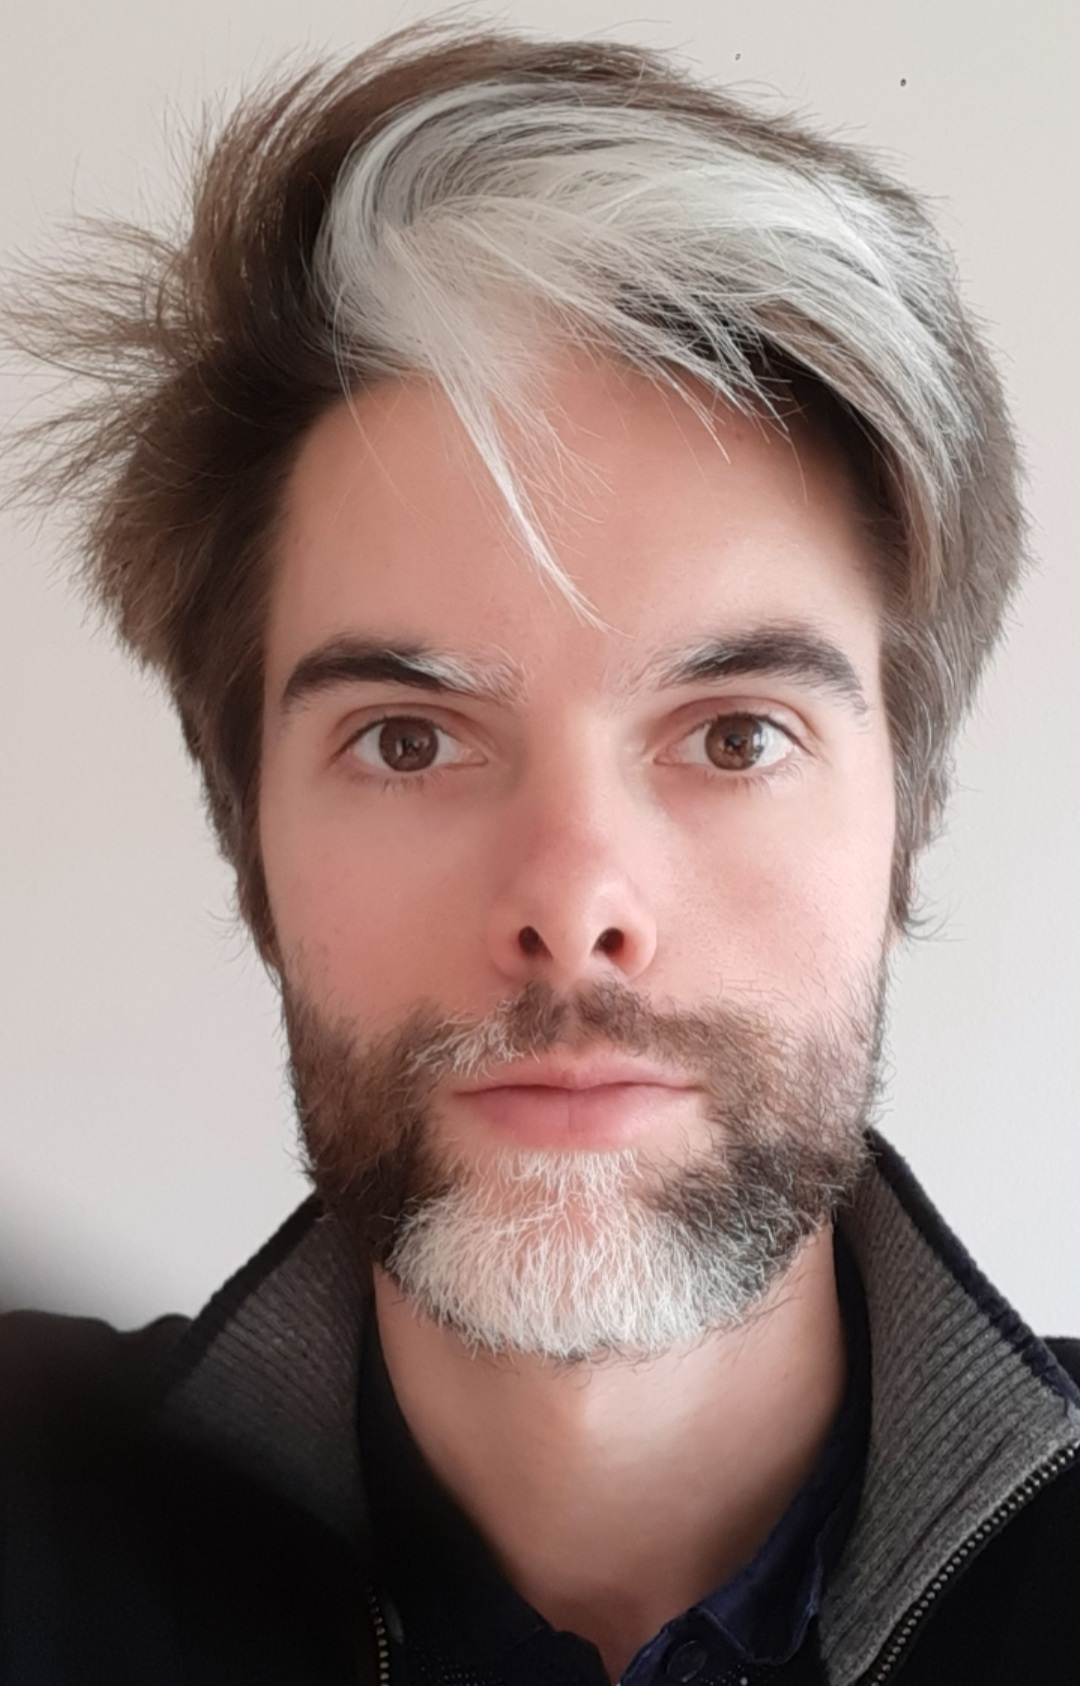
\includegraphics[width=0.65\textwidth]{photo3.jpg}\hfill\null

\vspace*{0.5ex} % Extra space after the picture

\headleft{Profile}

Theoretical physicist with over 8 years of extensive research experience in theoretical and computational plasma physics. 
My expertise lies in developing innovative theoretical models and performing complex simulations to understand plasma behavior in both laboratory and astrophysical environments. 

\headleft{Contact details}
\small % To fit more content
\MVAt\ {\small moreno\_quentin@numericable.fr} \\[0.4ex]
% \Mobilefone\ +420\,606\,782\,936 \\[0.5ex]
\Mobilefone\ +33\,628\,480\,516 \\[0.5ex]
\Mundus\ \href{https://kantmg.github.io/Quentin-s_portfolio/}{Portfolio} \\[0.1ex]
% \Letter\ 1542/32 Pujmanové Praha 4 CZ


\Letter\ 427 route de Broche\\
Saint Laurent des Hommes
\normalsize

\headleft{Personal information}
%Year of birth: \textbf{1861} \\[0.5ex]
Citizenship: \textbf{French} \\[0.5ex]
Family: \textbf{Single without children} \\[0.5ex]
Languages: \textbf{French (native)}, \textbf{English (fluent)}, , \textbf{Spanish (Intermediate)}

\headleft{Software Skills}
\begin{itemize}
\item Python
\item SQL
\item PowerBI
\item fortran95
\item Mathematica
\item LaTeX
\item MS Word, Excel, PowerPoint
% \item Communication and team collaboration
\end{itemize} 

\headleft{Scientific expertise}
\begin{itemize}
\item Plasma Instabilities
\item Shock formation
\item Laser plasma interaction
\item Kinetic Particle-in-cell code (\href{https://smileipic.github.io/Smilei/index.html}{SMILEI}/EPOCH)
\item Magneto-hydrodynamic AMR code (\href{https://flash.rochester.edu/site/flashcode/}{FLASH})
\item Machine learning
\end{itemize} 

% \headleft{Publications}
% \begin{itemize}
% \item 14 publications in peer-reviewed journals (5 as first author)
% \item h-index: 6 (from scopus)
% \end{itemize} 

\end{minipage}%
\kern0.09\textwidth\relax%%Right margin provided explicitly to stretch the colourbox
}
\end{minipage}% Right column
\hskip2.5em% Left margin for the white area
\begin{minipage}[t]{0.56\textwidth}
\setlength{\parskip}{0.8ex}% Adds spaces between paragraphs; use \\ to add new lines without this space. Shrink this amount to fit more data vertically

\vspace{2ex}

\headright{Experience}


\textsc{Postdoctoral fellow} at \textit{ELI-beamlines}  \dates{2019.01--2023.12} \\

\smaller{Theoretical studies on radiative/adiabatic shocks in a context relevant to laboratory astrophysics.}

\begin{itemize}
\item  \small{Designed analytical self-similar models.}

\item  \small{Realized Magneto-Hydrodynamic AMR simulations on large supercalculators.}

\item  \small{Created AMR simulations data visualization tools (matplotlib).}

\item  \small{Analyzed large datasets to confront analytical models with numerical simulations.}

\item  \small{Collaborated with cross-functional teams to design complex laboratory experiment to assess effectiveness of analytical models.}

\item  \small{Published findings in peer-reviewed journals and presented at international conferences.}

\end{itemize}


\smaller{Conducted numerical analysis to support various research projects.}


\smaller{Supervised a first year master student during 3 months.}\\

\is % Item spacing -- defined in the preamble
\textsc{Phd Student} at \textit{Bordeaux University.}  \dates{2015.10--2018.12} \\

\smaller{Theoretical studies on plasma instabilities that can lead to collisionless shocks in a context relevant to laboratory astrophysics.}
\begin{itemize}
\item  \small{Designed analytical models.}

\item  \small{Realized Particle-In-Cell (PIC) simulations on large supercalculators.}

\item  \small{Created PIC simulations data visualization tools (matplotlib).}

\item  \small{Analyzed large datasets to confront analytical models with numerical simulations.}

\item  \small{Collaborated with cross-functional teams to design complex laboratory experiment to assess effectiveness of analytical models.}

\item  \small{Published findings in peer-reviewed journals and presented at international conferences.}

\end{itemize}



\smaller{Course examiner} at \textit{Bordeaux University}
\begin{itemize}
\item  \small{Teaching experience from Bachelor to master degree.}\\
\end{itemize}


\is % Item spacing -- defined in the preamble
\textsc{Publications}\\
\smaller{13 publications in peer-reviewed journals}\\
\smaller{h-index: 7 (from \href{https://www.researchgate.net/profile/Quentin-Moreno}{researchgate}) }



\headright{Education at Bordeaux University}


\textsc{Doctoral Degree:} Astrophysics,plasma and nuclear \dates{2015--2018} \\
\smaller{Thesis title: \textit{Non-relativistic collisionless shocks in
Laboratory Astrophysics.}}
% \smaller{Econometric analysis, survival analysis, panel and time-series models.}
\is
\textsc{Master's Degree:} Theoretical physics \dates{2013--2015} \\
\smaller{Astrophysics, Statistical physics, numerical methods}

\is
\textsc{Bachelor’s Degree:} Theoretical physics \dates{2010--2013}

% 
% \headright{Intern experience}
% 
% 
% \textsc{Study of electron heating as part of the dynamics of
% collisionless shocks.}
% \textit{CELIA laboratory} \dates{2014--2015} \\
% \smaller{Particle-in-cell simulation, Plasma Instabilities, Laser-plasma interaction}
% 
% \is
% \textsc{Study of complex molecules in a star formation region}
% \textit{Bordeaux observatory} \dates{2013--2014} \\
% \smaller{ALMA data processing, spectral confusion analysis}
% 
% \is
% \textsc{Study of the evolution of surface tension at the nanoscale by analyzing
% the evaporation of drops from a critical mixture.}
% \textit{LOMA laboratory} \dates{2012--2013} \\
% \smaller{Deformation of a liquid surface by laser, experimental internship}

% \headright{Hobbies}
% 
% \textit{Music:} imitating birds on the banjo, composing and decomposing (morally).
% 
% \textit{Poetry:} inventing rhymes, surreal art.
% 
% \textit{Miscellaneous:} zoology, mycology, trainspotting, 1930s horror films.
\end{minipage}

\end{document}
